%& -shell-escape -enable-write18
\documentclass{standalone}
\usepackage{tikz}
%\usepackage{caption}
\usetikzlibrary{external}
\usetikzlibrary{shapes,arrows}
%\newcommand{mynodename}[#1]{\mathrm{#1}}
%\newcommand{mylabelleft}[#2]{label={[font=\fontsize{#1}{#1}\selectfont]above left:mynodename{#2}}}
\begin{document}
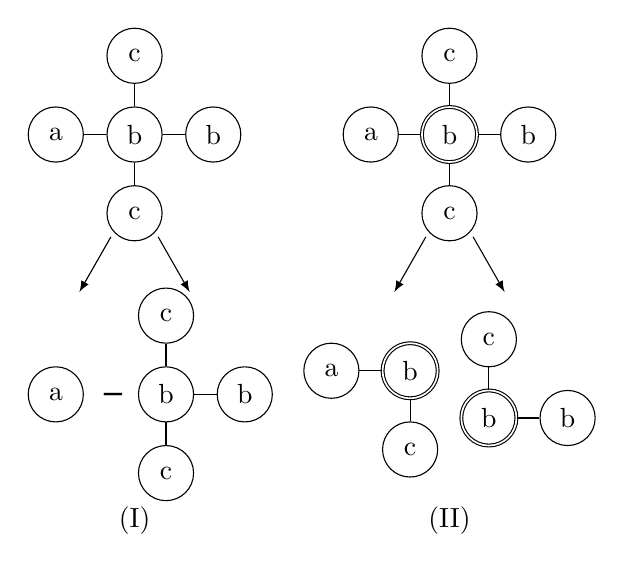
\begin{tikzpicture}[scale=1.0]
%[every node/.style={draw,circle}]
\tikzstyle{every node}=[draw,shape=circle,minimum size=0.7cm];
\tikzstyle{mylabels}=[font=\fontsize{7}{7}\selectfont];
\tikzstyle{line} = [draw,-latex]


%\draw[help lines] (-1.0,-6.0) grid (12.0,6.0);
\begin{scope}[shift={(0,0)}]%upper row set
	\begin{scope}[shift={(1,4.0)}]%upper row left
  		\node (a1) at (0,0) {a};
 		\node (b1) at (1,0) {b};
  		\node (b2) at (2,0) {b};
  		\node (c1) at (1,1) {c};
  		\node (c2) at (1,-1) {c};
  
		\foreach \from/\to in {a1/b1,b1/b2,b1/c1, b1/c2}
   		 \draw (\from) -- (\to);
	\end{scope}
	\begin{scope}[shift={(5.0,4)}]%upper row right
 		 \node (a2) at (0,0) {a};
 		 \node[draw,double,shape=circle,minimum size=0.7cm] (b3) at (1,0) {b};
 		 \node (b4) at (2,0) {b};
		 \node (c3) at (1,1) {c};
 		 \node (c4) at (1,-1) {c};
  
	  	\foreach \from/\to in {a2/b3,b3/b4,b3/c3, b3/c4}
   		 \draw (\from) -- (\to);
	\end{scope}
\end{scope}%upper row set
\begin{scope}[shift={(0,0.7)}]% lower row set
	\begin{scope}[shift={(0,0)}] % lower row extreme left
		\node (a3) at (1,0) {a};
		\node [draw=none] (minus)      at   (1.6,0){\scalebox{2.5}[1.5]{ -} };%horizontal scaling with no vertical scaling
		\node [draw=none] (EdgeCutting) at (2.0,-1.6) { (I) };% edge cutting label
		\node [draw=none] (EdgeCutting) at (6.0,-1.6) { (II) };% edge cutting label
	\end{scope}
	\begin{scope}[shift={(2.4,0)}]%lower row second from left
  		\node (b5) at (0,0) {b};
 		\node (b6) at (1,0) {b};
		\node (c5) at (0,1) {c};
		\node (c6) at (0,-1) {c};
		
		
		\foreach \from/\to in {b5/b6,b5/c5, b5/c6}
			\draw (\from) -- (\to);
	\end{scope}
	\begin{scope}[shift={(4.5,.3)}]% lower row middle right
  		\node (a4) at (0,0) {a};
  		\node[draw,double,shape=circle,minimum size=0.7cm] (b7) at (1,0) {b};
  		\node (c7) at (1,-1) {c};
  
 		 \foreach \from/\to in {a4/b7,b7/c7}
   		 \draw (\from) -- (\to);
	\end{scope}% lower row middle right
	\begin{scope}[shift={(5.5,-.3)}]% lower row extreme right
		\node[draw,double,shape=circle,minimum size=0.7cm] (b8) at (1,0) {b};
		\node (b9) at (2,0) {b};
 		\node (c8) at (1,1) {c};
 	 		\foreach \from/\to in {b8/b9,b8/c8}
	    		\draw (\from) -- (\to);
	\end{scope}% lower row extreme right
\end{scope}%lower row set
\begin{scope}[shift={(0,0)}]% the arrows set
	\begin{scope}[shift={(1.8,2.7)}]%the left arrows
		\path[line] (-0.1,0) -- (-0.5,-0.7);
		\path[line] (0.5,0) -- (0.9,-0.7);
	\end{scope}
	\begin{scope}[shift={(5.8,2.7)}]%the right arrows
		\path[line] (-0.1,0) -- (-0.5,-0.7);
		\path[line] (0.5,0) -- (0.9,-0.7);
	\end{scope}
\end{scope}
\end{tikzpicture}
\end{document}
